\documentclass[fsharpNotes.tex]{subfiles}
\graphicspath{ {figures/} }

\begin{document}
\chapter{Using F\# as a Calculator}
\label{chap:calculator}

%\begin{minipage}{\linewidth}
%  \centering
 % \includegraphics[width=\linewidth]{constantsNOperators}
%\end{minipage}
%\newpage
\abstract[figures/numbersCharsNStrings]{
  \begin{figure} % We want the figure on the first page with the chapter title
    \centering
    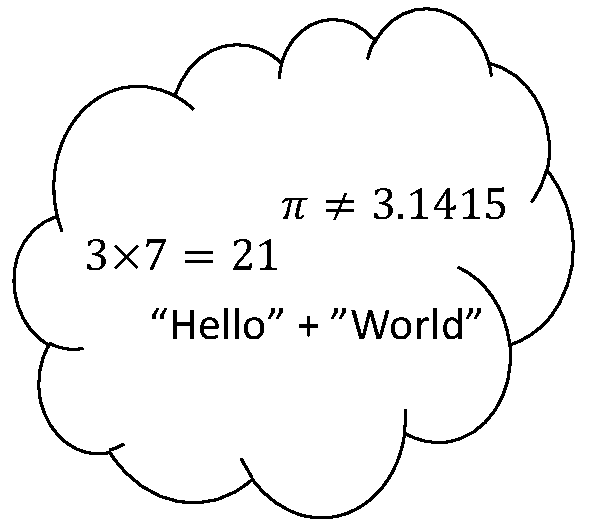
\includegraphics[width=0.6\textwidth]{constantCloud} % for some reason, it does not want to read the pdf-file
    \caption{The basis of F\# are constants and expressions}
    \label{fig:numbersCharsNStrings}
  \end{figure}
In the previous chapter, we introduced some key F\# programming tools and concepts without going into depth on opportunities and limitations. In the following chapters, we will dive deeper into methods for solving problems by writing programs, and what facilities are available in F\# to express these solutions. As a first step, we must acquaint ourselves with the basic building blocks of basic types, constants, and operators, and this chapter includes
  \begin{itemize}
  \item An introduction to the basic types and how to write constants of those types.
  \item Arithmetic of basic operations.
  \end{itemize}
  with these tools, you will be able to evaluate expressions as if F\# were a simple calculator. Examples of problems, you will be able to solve after reading this chapter, is:
  \begin{itemize}
  \item What is the result of $3\cos(4*\pi/180)+4\sin(4*\pi/180)$.
  \item Calculate how many characters are there in the text string ``Hello World!''.
  \item What is the ASCII value of the character 'J'.
  \item How to convert between whole and binary numbers.
  \end{itemize}
}
%Talking about programs and programming languages we make a distinction between the language's \idx{syntax}, which describes what are legal expressions and statements, and the \idx{semantics} of an expression and a statement, which describes what is meant. This is analog to human languages, where how nouns, verbs, etc. may be placed in relation to each describes the syntax of a sentence, while the meaning of a sentence is its semantics. Basic elements of F\#'s syntax are literals, which is a fixed value like the number 3.

\section{Literals and Basic Types}
All programs rely on the processing of data, and an essential property of data is its \idx{type}. A \idx{literal} is a fixed value like the number 3, and if we type the number \lstinline!3! in an interactive session at the input prompt, then F\# responds as shown in \Cref{firstType}.
%
\fsOutput{firstType}{Typing the number 3.}
%
What this means is that F\# has inferred the type to be \idx[int@\lstinline{int}]{\lstinline{int}} and bound it to the identifier \idx[it@\lstinline{it}]{\lstinline{it}}. For more on binding and identifiers see \Cref{chap:let}. Types matter, since the operations that can be performed on integers, are quite different from those that can be performed on, e.g., strings. Therefore, the number 3 has many different representations as shown in \Cref{typeMatters}.
%
\fsOutput{typeMatters}{Many representations of the number 3 but using different types.}
%
Each literal represents the number 3, but their types are different, and hence they are quite different values. The types \lstinline!int! for integer numbers, \idx[float@\lstinline{float}]{\lstinline{float}} for floating point numbers, \idx[bool@\lstinline{bool}]{\lstinline{bool}} for Boolean values, \idx[char@\lstinline{char}]{\lstinline{char}} for characters, and \idx[string@\lstinline{string}]{\lstinline{string}} for strings of characters are the most common types of literals. A table of all \idx{basic types} predefined in F\# is given in \Cref{tab:primitiveTypes}.\idxss{unit@\lstinline{unit}}\idxss{obj@\lstinline{obj}}\idxss{exn@\lstinline{exn}}
\begin{table}
  \centering
  \rowcolors{2}{oddRowColor}{evenRowColor}
  \begin{tabularx}{\textwidth}{|l|l|>{\raggedright\arraybackslash}X|}
    \hline
    \rowcolor{headerRowColor} Metatype & Type name & Description\\
    \hline
    Boolean & \underline{\keyword{bool}} & Boolean values true or false \\
    \hline
    Integer & \underline{\keyword{int}} & Integer values from -2,147,483,648 to 2,147,483,647 \\
             & \keyword{byte} &Integer values from 0 to 255\\
             & \keyword{sbyte} &Integer values from -128 to 127\\
             & \keyword{int8} &Synonymous with sbyte\\
             & \keyword{uint8} &Synonymous with byte\\
             & \keyword{int16} &Integer values from -32768 to 32767\\
             & \keyword{uint16} &Integer values from 0 to 65535\\
             & \keyword{int32} &Synonymous with int\\
             & \keyword{uint32} & Integer values from 0 to 4,294,967,295\\
             & \keyword{int64} &Integer values from -9,223,372,036,854,775,808 to 9,223,372,036,854,775,807\\
             & \keyword{uint64} &Integer values from 0 to 18,446,744,073,709,551,615\\
             %& bignum &Integer not limited to 64 bits\\
             %& nativeint &A native pointer as a signed integer\\
            % & unativeint &A native pointer as an unsigned integer\\
    \hline
    Real &\underline{\keyword{float}} & 64-bit IEEE 754 floating point value from $-\infty$ to $\infty$\\
             & \keyword{double} & Synonymous with float\\
             & \keyword{single} &A 32-bit floating point type\\
             & \keyword{float32} &Synonymous with single\\
             & \keyword{decimal} &A floating point data type that has at least 28 significant digits\\
    \hline
    Character &\underline{\keyword{char}} &Unicode character\\
             &\underline{\keyword{string}} & Unicode sequence of characters\\
    \hline
    None &\underline{\keyword{unit}} & The value ()\\
    \hline
    Object &\underline{\keyword{obj}} & An object\\
    \hline
    Exception &\underline{\keyword{exn}} & An exception\\
    \hline
  \end{tabularx}
  \caption{List of some of the basic types. The most commonly used types are underlined. For a description of integer see Appendix~\ref{sec:binary}, for floating point numbers see Appendix~\ref{sec:floatingPoint}, for ASCII and Unicode characters see Appendix~\ref{sec:characterSets}, for objects see \Cref{chap:oop}, and for exceptions see \Cref{chap:errors}.}
  \label{tab:primitiveTypes}
\end{table}
In addition to these built-in types, F\# is designed such that it is easy to define new types. 

Humans like to use the \idx{decimal number} system for representing numbers. Decimal numbers are \idx{base}~10, which means that a value is represented as two sequences of decimal digits separated by a \idx{decimal point}, where each \idx{digit} $d$ has a position and a value $d \in \{0,1,2,\ldots,9\}$. The part before the decimal point is called the \idx{whole part} and the part after is called the \idx{fractional part} of the number. An \idx{integer} is a number with only a whole part and neither a decimal point nor a fractional part. As an example \lstinline!35.7! is a decimal number, whose value is $3\cdot 10^1+5\cdot 10^0+7\cdot 10^{-1}$, and \lstinline!128! is an integer, whose value is $1\cdot 10^2+2\cdot 10^1+8\cdot 10^{0}$. In F\#, a decimal number is called a \idx{floating point number}.  Floating point numbers may alternatively be given using \idx{scientific notation}, such as \lstinline!3.5e-4! and \lstinline!4e2!, where the \lstinline!e!-notation is translated to a value as \lstinline!3.5e-4!~$=3.5\cdot 10^{-4} = 0.00035$, and \lstinline!4e2!~$=4\cdot 10^2=400$.

The basic unit of information in almost all computers is the binary digit or \idx{bit} for short. Internally, programs and data are all represented as bits, hence F\# has strong support for binary numbers. A \idx{binary number} consists of a sequence of binary digits separated by a decimal point, where each digit can have values $b \in \{0,1\}$, and the base is $2$. E.g., the binary number $101.01_2 = 1\cdot 2^2+0\cdot 2^1+1\cdot 2^0+0\cdot 2^{-1}+1\cdot 2^{-2}=5.25$. Subscripts are often used to indicate the base of a number, e.g., $101.01_2$ and $101.01_{10}$ are different numbers. Since base 10 is so common, the subscript for base 10 numbers is often omitted. 

Binary numbers are closely related to \idx[octal number]{octal} and \idx[hexadecimal number]{hexadecimal numbers}. Octals use 8 as their basis and hexadecimals use 16 as their basis. Each octal digit can be represented by exactly three bits, and each hexadecimal digit can be represented by exactly four bits. The hexadecimal digits use \lstinline!0!--\lstinline!9! to represent the values 0--9 and \lstinline!a!--\lstinline!f! in lower or alternatively upper case to represent the values 10-15.  Thus, Octals and hexadecimals conveniently serve as shorthand for the much longer binary representation. As examples, the octal number \lstinline!37!$_8$ is $3\cdot 8^1+7\cdot 8^0=31$, and the hexadecimal number \lstinline!f3!$_{16}$ is $15\cdot 16^1+3\cdot 16^0=243$. 

To denote integers in bases different than 10, F\# uses the prefix '0b' for binary, '0o' for octal, and '0x' for hexadecimal numbers.  For example, the value $367_{10}$ may be written as an integer \lstinline!367!, as a binary number \lstinline!0b101101111!, as an octal number \lstinline!0o557!, and as a hexadecimal number \lstinline!0x16f!. In F\#, the character sequences \lstinline!0b12! and \lstinline!ff! are not recognized as numbers.

A \idx{character} is a \idx{Unicode} \idx{code point}, and character literals are enclosed in single quotation marks. Appendix~\ref{sec:unicode} contains more details on code points.\spec{Spec-4.0 p.28: \texttt{char-char} is missing option \texttt{unicodegraph-long} } The character type in F\# is denoted \idx[char@\lstinline{char}]{\keyword{char}}.  Examples of characters are 'a', 'D', '3', and examples of non-characters are '23' and 'abc'. Some characters, such as the tabulation character, do not have a visual representation. These can still be represented as a character using \idx{escape sequences}. A character escape sequence starts with \lexeme{\\} followed by letter for simple escapes such as \lstinline{\t} for tabulation and \lstinline{\n} for newline. Escape sequences can also be a numerical representation of a code point, and three versions exist: The trigraph \lstinline|\DDD|, where \lstinline{D} is a decimal digit, is used to specify the first 256 code points, the hexadecimal escape codes \lstinline|\uXXXX|, where \lstinline{X} is a hexadecimal digit, is used to specify the first 65536 code points, and \lstinline|\UXXXXXXXX| is used to specify any of the approximately $4.3\cdot 10^9$ possible code points. All escape sequences are shown in \Cref{tab:escapeChar}.
%
\begin{table}
  \centering
  \rowcolors{2}{oddRowColor}{evenRowColor}
  \begin{tabular}{|c|p{0.2\textwidth}|p{0.57\textwidth}|}
    \hline
    \rowcolor{headerRowColor} Character& Escape sequence & Description\\
    \hline
    BS &\lstinline|\b|& Backspace\\
    LF &\lstinline|\n|&Line feed\\
    CR &\lstinline|\r|&Carriage return\\
    HT &\lstinline|\t|&Horizontal tabulation\\
    \textbackslash &\lstinline|\\|&Backslash\\
     " &\lstinline|\"|&Quotation mark\\
    ' &\lstinline|\'|&Apostrophe\\
    BEL&\lstinline|\a|& Bell\\
    FF&\lstinline|\f|&Form feed\\
    VT &\lstinline|\v|&Vertical tabulation\\
    &\lstinline|\uXXXX|, \lstinline|\UXXXXXXXX|, \lstinline|\DDD|&Unicode character ('X' is any hexadecimal digit, and 'D' is any decimal digit)\\
    \hline
  \end{tabular}
  \caption{Escape characters. The escape code \inlinecode{\textbackslash DDD} is sometimes called a tricode.}
  \label{tab:escapeChar}
\end{table}
%
Examples of \keyword{char} representations of the letter 'a' are: \lstinline{'a'}, \lstinline{'\097'}, \lstinline{'\u0061'}, \lstinline{'\U00000061'}.

A \idx{string} is a sequence of characters enclosed in double quotation marks.  Examples are \lstinline{"a"}, \lstinline{"this is a string"}, and \lstinline{"-&#\@"}. Note that the string \lstinline{"a"} and the character \lstinline{'a'} are not the same. Some strings are so common that they are given special names: One or more spaces \lstinline{" "} is called \idx{whitespace}, and both \lstinline{"\n"} and \lstinline{"\r\n"} are called \idx{newline}.  The escape-character \lexeme{\\} may be used to break a line in two. This and other examples are shown in \Cref{stringLiterals}.
%
\fsOutput{stringLiterals}{Examples of string literals.}
%
Note that the response from \lstinline[language=console]{fsharpi} is shown in double quotation marks, but this is not part of the string. 

F\# supports \idx[literal type]{literal types}, where the type of a literal is indicated as a prefix or suffix as shown in \Cref{tab:literalTypes}.\idxss{int32@\lstinline{int32}}\idxss{uint32@\lstinline{uint32}}\idxss{byte@\lstinline{byte}}\idxss{uint8@\lstinline{uint8}}\idxss{byte@\lstinline{byte[]}}\idxss{sbyte@\lstinline{sbyte}}\idxss{int8@\lstinline{int8}}\idxss{int16@\lstinline{int16}}\idxss{uint16@\lstinline{uint16}}\idxss{int64@\lstinline{int64}}\idxss{uint64@\lstinline{uint64}}\idxss{double@\lstinline{double}}\idxss{single@\lstinline{single}}\idxss{float32@\lstinline{float32}}\idxss{decimal@\lstinline{decimal}}
\begin{table}
  \centering
  %\begin{tabularx}{\linewidth}{|>{\hsize=.6\hsize}X|>{\hsize=1.4\hsize}X|>{\hsize=1\hsize}X|}
  \rowcolors{2}{oddRowColor}{evenRowColor}
  \setlength{\tabcolsep}{3pt}
  \begin{tabular}{|p{24mm}|p{25mm}|p{28mm}|p{27mm}|}
    \hline
    \rowcolor{headerRowColor} Type & syntax & Examples & Value \\
    \hline
    {\keyword{int}}, {\keyword{int32}}          
                                   & {\lstinline[language=syntax, keywords={}]!<*int | xint*>!}\newline
                                     {\lstinline[language=syntax, keywords={}]!<*int | xint*>l!}
                                            & {\lstinline!3!}, {\lstinline!0x3!}\newline
                                              {\lstinline!3l!}, {\lstinline!0x3l!}
                                                       & 3\\
    {\keyword{uint32}}                                 
                                   & {\lstinline[language=syntax, keywords={}]!<*int | xint*>u!}\newline
                                     {\lstinline[language=syntax, keywords={}]!<*int | xint*>ul!}
                                            & {\lstinline!3u!}\newline
                                              {\lstinline!3ul!}
                                                       & 3 \\
    {\keyword{byte}}, {\keyword{uint8}}       
                                   & {\lstinline[language=syntax, keywords={}]!<*int | xint*>uy!}\newline
                                     {\lstinline[language=syntax, keywords={}]!'<*char*>'B!}
                                            & {\lstinline!97uy!}\newline
                                                       {\lstinline!'a'B!} 
                                                       & 97 \\
    {\keyword{byte[]}}
                                   & {\lstinline[language=syntax, keywords={}]!"<*string*>"B!}\newline
                                     {\lstinline[language=syntax, keywords={}]!@"<*string*>"B!}
                                            & {\lstinline!"a\n"B!}\newline
                                                       {\lstinline!@"a\n"B!} 
                                                       & [|97uy; 10uy|]\newline
                                                         [|97uy; 92uy; 110uy|] \\
    {\keyword{sbyte}}, {\keyword{int8}}
                                   & {\lstinline[language=syntax, keywords={}]!<*int | xint*>y!}
                                            & {\lstinline!3y!}
                                                       & 3 \\
    {\keyword{int16}}
                                   & {\lstinline[language=syntax, keywords={}]!<*int | xint*>s!}
                                            & {\lstinline!3s!}
                                                       & 3 \\
    {\keyword{uint16}}
                                   & {\lstinline[language=syntax, keywords={}]!<*int | xint*>us!}
                                            & {\lstinline!3us!}
                                                       & 3 \\
    {\keyword{int64}}
                                   & {\lstinline[language=syntax, keywords={}]!<*int | xint*>L!}
                                            & {\lstinline!3L!}
                                                       & 3 \\
    {\keyword{uint64}}
                                   & {\lstinline[language=syntax, keywords={}]!<*int | xint*>UL!}\newline
                                     {\lstinline[language=syntax, keywords={}]!<*int | xint*>uL!}   
                                            & {\lstinline!3UL!}\newline
                                              {\lstinline!3uL!}  
                                                       & 3 \\
    % {\keyword{bignum}}$^*$                      & {\lstinline[language=syntax, keywords={}]!dInt "I"!}                                        & {\lstinline!3I!} & 3 \\
    % {\keyword{nativeint}}                            & {\lstinline[language=syntax, keywords={}]!(dInt | xInt) "n"!}                           & {\lstinline!3n!} & 3 \\
    % {\keyword{unativeint}}                          & {\lstinline[language=syntax, keywords={}]!(dInt | xInt) "un"!}                         & {\lstinline!3un!} & 3 \\
    {\keyword{float}}, {\keyword{double}}
                                   & {\lstinline[language=syntax, keywords={}]!<*float*>!}\newline
                                     {\lstinline[language=syntax, keywords={}]!<*xint*>LF!}
                                            & {\lstinline!3.0!}\newline
                                              {\lstinline!0x013LF!} 
                                                       & 3.0\newline
                                                         9.387247271e-323 \\
    {\keyword{single}}, {\keyword{float32}} 
                                   & {\lstinline[language=syntax, keywords={}]!<*float*>F!}\newline
                                     {\lstinline[language=syntax, keywords={}]!<*float*>f!}\newline
                                     {\lstinline[language=syntax, keywords={}]!<*xint*>lf!} 
                                   & {\lstinline!3.0F!}\newline
                                     {\lstinline!3.0f!}\newline
                                     {\lstinline!0x013lf!}
                                                       & 3.0\newline
                                                         3.0 \newline
                                                         4.4701421e-43f \\
    {\keyword{decimal}}  
                                   & {\lstinline[language=syntax, keywords={}]!<*float | int*>M!}\newline
                                     {\lstinline[language=syntax, keywords={}]!<*float | int*>m!}
                                            & {\lstinline!3.0M!}, {\lstinline!3M!}\newline
                                              {\lstinline!3.0m!}, {\lstinline!3m!} 
                                                       & 3.0  \\
    {\keyword{string}} 
                                   & {\lstinline[language=syntax, keywords={}]!"<*string*>"!}\newline
                                     {\lstinline[language=syntax, keywords={}]!@"<*string*>"!}\newline
                                     {\lstinline[language=syntax, keywords={}]!"""<*string*>"""!}
                                            & {\lstinline!"\"quote\".\n"!}\newline
                                              {\lstinline!@"""quote"".\n"!}\newline
                                              {\lstinline!""""quote".\n"""!}
                                                       & "quote".<newline>\newline
                                                         "quote".\textbackslash n.\newline
                                                         "quote".\textbackslash n\\
    \hline
  \end{tabular}
  % \end{tabularx}
  \caption{List of literal types. The syntax notation {\lstinline[language=syntax, keywords={}]!<**>!} means that the programmer replaces the brackets and content with a value of the appropriate form. The \lstinline[language=syntax, keywords={}]{<*xint*>} is one of the integers on hexadecimal, octal, or binary forms such as \lstinline{0x17}, \lstinline{0o21}, and \lstinline{0b10001}.  The \lstinline{[| |]} brackets means that the value is an array, see \Cref{sec:arrays} for details.
    % The \lstinline![]! notation is for lists, see \Cref{chap:lists}. $^*$\lstinline[language=ebnf]!bignum! is not a basic type and does not yet have an implementation for \lstinline[language=ebnf]!dInt ("Q"|"R"|"Z"|"N"|"G")! in Mono.
  }
  \label{tab:literalTypes}
\end{table}
%The table uses a simple syntax notation such that {\lstinline[language=syntax, keywords={}]!<*integer or hexadecimal*>UL!} means that the user supplies an integer or a hexadecimal number followed by the characters 'UL'.


The literal type is closely connected to how the values are represented internally. For example, a value of type \keyword{int32} uses 32 bits and can be both positive and negative, while a \keyword{uint32} value also uses 32 bits, but is unsigned. A \keyword{byte} is an 8-bit number, and \keyword{sbyte} is a signed 8-bit number. Values of type \keyword{float} use 64 bits, while \keyword{float32} only uses 32 bits. The number of bits used to represent numbers directly relates to the range and precision these types can represent. This is summarized in \Cref{tab:primitiveTypes} and discussed in more detail in \Cref{app:numbers}. String literals may be \idx{verbatim} by the @-notation or triple double quotation marks, meaning that the escape sequences are not converted to their code point. The two types of string verbatim treat quotation marks differently, as illustrated in the table. Further examples are shown in \Cref{namedLiterals}.
%
\fsOutput{namedLiterals}{Named and implied literals.}
%
%
%\fsOutput{stringVerbatim}{Examples of a string literal.}
%
%For strings containing double quotation marks, verbatim literals have 2 possible notations, either use the @-notation and escape double quotation marks with an extra double quotation mark or use triple double quotation marks. \advice{The triple double quotation marks notation may not contain substrings that are triple double quotation marks, and thus @-notation is preferred.}

Many basic types are compatible, and the type of a literal may be changed by \idx{typecasting}. An example of casting to a \keyword{float} is shown in \Cref{upcastingInt}.
%
\fsOutput{upcastingInt}{Casting an integer to a floating point number.}
% 
When \lstinline|float| is given an argument, then it acts as a function rather than a type, and for the integer \lstinline|3| it returns the floating point number \lstinline|3.0|.  For more on functions see \Cref{chap:let}. Boolean values are often treated as integer values 0 and 1, but no short-hand function names exist for their conversions. Instead, use functions from the \lstinline{System.Convert} family of functions, as demonstrated in \Cref{castingBooleans}.
%
\fsOutput{castingBooleans}{Casting booleans.}
% 
Here \lstinline|System.Convert.ToBoolean| is the identifier of a function \lstinline|ToBoolean|, which is a \idx{member} of the \idx{class} \lstinline|Convert| that is included in the \idx{namespace} \lstinline|System|. Namespaces, classes, and members will be discussed in \Cref{chap:modules}.

Typecasting is often a destructive operation, e.g., typecasting a \lstinline!float! to \lstinline{int} removes the fractional part without rounding as shown in \Cref{downcasting}.
%
\fsOutput{downcasting}{Fractional part is removed by downcasting.}
%
Here we typecasted to a lesser type, in the sense that the set of integers is a subset of floating point numbers, and this is called \idx[downcast]{downcasting}. The opposite is called \idx[upcast]{upcasting} and is often non-destructive, as \Cref{upcastingInt} showed. Since floating point numbers are a superset of integers, the value is retained. As a side note, \idx{rounding} a number $y.x$, where $y$ is the \idx{whole part} and $x$ is the \idx{fractional part}, is the operation of mapping numbers in the interval $y.x \in [y.0,y.5)$ to $y$, and those in $y.x\in [y.5,y+1)$ to $y+1$. This can be performed by downcasting, as shown in \Cref{rounding}.
%
\fsOutput{rounding}{Rounding by modified downcasting.}
%
I.e., $357.6+0.5=358.1$ and removing the fractional part by downcasting results in $358$, which is the correct answer.

\section{Operators on Basic Types}
Expressions are the basic building block of all F\# programs, and this section will discuss operator expressions on basic types. 
A typical calculation, such used in \Cref{rounding}, is \begin{equation}
  \underbrace{357.6}_{\text{operand}}\quad\underbrace{+}_{\text{operator}}\quad\underbrace{0.5}_{\text{operand}}
\end{equation}
is an example of an arithmetic \idx{expression}, and the above expression consists of two \idx[operand]{operands} and an \idx{operator}. Since this operator takes two operands, it is called a \idx{binary operator}. The expression is written using \idx{infix notation}, since the operands appear on each side of the operator.

In order to discuss general programming structures, we will use simplified language to describe valid syntactical structures. In this simplified language, the syntax of basic binary operators is shown in the following.
%
\begin{verbatimwrite}{\ebnf/binaryOperator.ebnf}
<*expr*><*op*><*expr*>
\end{verbatimwrite}
\syntax{\ebnf/binaryOperator.ebnf}{Syntax for a binary expression.}
%
Here \lstinline[language=syntax]{<*expr*>} is any expression supplied by the programmer, and \lstinline[language=syntax]{<*op*>} is a binary infix operator. F\# supports a range of arithmetic binary infix operators on its built-in types, such as addition, subtraction, multiplication, division, and exponentiation, using the \lexeme{+}, \lexeme{-}, \lexeme{*}, \lexeme{/}, \lexeme{**} lexemes, respectively. Not all operators are defined for all types, e.g., addition is defined for integer and float types as well as for characters and strings, but multiplication is only defined for integer and floating-point types. A complete list of built-in operators on basic types is shown in \Cref{tab:preNInfixOperators} and~\ref{tab:comparisonOperators}, and a range of mathematical functions is shown in \Cref{tab:arithmeticFunctions}.
%
\begin{table}
  \centering
  \rowcolors{2}{oddRowColor}{evenRowColor}
  \begin{tabularx}{\linewidth}{|c|c|c|c|c|c|l|l|>{\raggedright\arraybackslash}X|}
    \hline
    \rowcolor{headerRowColor} \rotatebox{90}{Operator} & \rotatebox{90}{\lstinline!bool!}& \rotatebox{90}{\lstinline!ints!}& \rotatebox{90}{\lstinline!floats!}& \rotatebox{90}{\lstinline!char!}& \rotatebox{90}{\lstinline!string!} & Example & Result &Description\\
    \hline
    \lstinline!+!& & \checkmark & \checkmark & \checkmark & \checkmark & \lstinline!5 + 2!&\lstinline!7!&Addition\\
    \hline
    \lstinline!-!& & \checkmark & \checkmark & & & \lstinline!5.0 - 2.0!&\lstinline!3.0!&Subtraction\\
    \hline
    \lstinline!*!& & \checkmark & \checkmark & & & \lstinline!5 * 2!&\lstinline!10!&Multiplication\\
    \hline
    \lstinline!/!& & \checkmark & \checkmark & & & \lstinline!5.0 / 2.0!&\lstinline!2.5!&Division\\
    \hline
    \lstinline!\%!& & \checkmark & \checkmark & & & \lstinline!5 \% 2!&\lstinline!1!&Remainder\\
    \hline
    \lstinline!**!& & & \checkmark & & & \lstinline!5.0 ** 2.0!&\lstinline!25.0!&Exponentiation\\
    \hline
    \lstinline!+!& & \checkmark & \checkmark & & &\lstinline!+3!&\lstinline!3!&identity\\
    \hline
    \lstinline!-!& & \checkmark & \checkmark & & &\lstinline!-3.0!&\lstinline!-3.0!&negation\\
    \hline
    \lstinline!\&\&!& \checkmark & & & & & \lstinline!true \&\& false!&\lstinline!false!&boolean and\\
    \hline
    \lstinline!||!& \checkmark & & & & & \lstinline!true || false!&\lstinline!true!&boolean or\\
    \hline
    \lstinline!not!& \checkmark & & & & &\lstinline!not true!&\lstinline!false!&boolean negation\\
    \hline
    \lstinline!\&\&\&!& & \checkmark & & & & \lstinline!0b101 \&\&\& 0b110!&\lstinline!0b100!&bitwise boolean and\\
    \hline
    \lstinline!|||!& & \checkmark & & & & \lstinline!0b101 ||| 0b110!&\lstinline!0b111!&bitwise boolean or\\
    \hline
    \lstinline!\^\^\^!& & \checkmark & & & & \lstinline!0b101 \^\^\^ 0b110!&\lstinline!0b011!&bitwise boolean exclusive or\\
    \hline
    \lstinline!<<<!& & \checkmark & & & & \lstinline!0b110uy <<< 2!&\lstinline!0b11000uy!&bitwise left shift\\
    \hline
    \lstinline!>>>!& & \checkmark & & & & \lstinline!0b110uy >>> 2!&\lstinline!0b1uy!&bitwise right shift\\
    \hline
    \lstinline!\~\~\~!& & \checkmark & & &&\lstinline!\~\~\~0b110uy!&\lstinline!0b11111001uy!&bitwise boolean negation\\
    \hline
  \end{tabularx}
  \caption{Arithmetic operators on basic types. Ints and floats means all built-in integer and float types. Note that for the bitwise operations, digits \lstinline{0} and \lstinline{1} are taken to be \lstinline{true} and \lstinline{false}.}
  \label{tab:preNInfixOperators}
\end{table}
%
\begin{table}
  \centering
  \rowcolors{2}{oddRowColor}{evenRowColor}
  \begin{tabularx}{\linewidth}{|c|c|c|c|c|c|l|l|X|}
    \hline
    \rowcolor{headerRowColor} \rotatebox{90}{Operator} & \rotatebox{90}{\lstinline!bool!}& \rotatebox{90}{\lstinline!ints!}& \rotatebox{90}{\lstinline!floats!}& \rotatebox{90}{\lstinline!char!}& \rotatebox{90}{\lstinline!string!} & Example & Result &Description\\
    \hline
    \lstinline!<!& \checkmark & \checkmark & \checkmark & \checkmark & \checkmark & \lstinline!true < false!&\lstinline!false!&Less than\\
    \hline
    \lstinline!>!& \checkmark & \checkmark & \checkmark & \checkmark & \checkmark & \lstinline!5 > 2!&\lstinline!true!&Greater than\\
    \hline
    \lstinline!=!& \checkmark & \checkmark & \checkmark & \checkmark & \checkmark & \lstinline!5.0 = 2.0!&\lstinline!false!&Equal\\
    \hline
    \lstinline!<=!& \checkmark & \checkmark & \checkmark & \checkmark & \checkmark & \lstinline!'a' <= 'b'!&\lstinline!true!&Less than or equal\\
    \hline
    \lstinline!>=!& \checkmark & \checkmark & \checkmark & \checkmark & \checkmark & \lstinline!"ab" >= "cd"!&\lstinline!false!&Greater than or equal\\
    \hline
    \lstinline!<>!& \checkmark & \checkmark & \checkmark & \checkmark & \checkmark & \lstinline!5 <> 2!&\lstinline!true!&Not equal\\
    \hline
  \end{tabularx}
  \caption{Comparison operators on basic types. Types cannot be mixed, e.g., \lstinline!3<'a'! is a syntax error.}
  \label{tab:comparisonOperators}
\end{table}
\idxss{\lstinline{abs}}\idxss{\lstinline{acos}}\idxss{\lstinline{asin}}\idxss{\lstinline{atan}}\idxss{\lstinline{atan2}}\idxss{\lstinline{ceil}}\idxss{\lstinline{cos}}\idxss{\lstinline{cosh}}\idxss{\lstinline{exp}}\idxss{\lstinline{floor}}\idxss{\lstinline{log}}\idxss{\lstinline{log10}}\idxss{\lstinline{max}}\idxss{\lstinline{min}}\idxss{\lstinline{pown}}\idxss{\lstinline{round}}\idxss{\lstinline{sign}}\idxss{\lstinline{sin}}\idxss{\lstinline{sinh}}\idxss{\lstinline{sqrt}}\idxss{\lstinline{tan}}\idxss{\lstinline{tanh}}
%
\begin{table}
  \centering
  \begin{tabularx}{\linewidth}{|c|c|c|c|c|c|l|l|>{\raggedright\arraybackslash}X|}
    \hline
    \rowcolor{headerRowColor} \rotatebox{90}{Operator} & \rotatebox{90}{\lstinline!bool!}& \rotatebox{90}{\lstinline!ints!}& \rotatebox{90}{\lstinline!floats!}& \rotatebox{90}{\lstinline!char!}& \rotatebox{90}{\lstinline!string!} & Example & Result &Description\\
    \hline
    \lstinline!abs! & & \checkmark & \checkmark & & &\lstinline!abs -3! & \lstinline!3! & Absolute value\\
    \hline 
    \lstinline!acos! & & & \checkmark & & &\lstinline!acos 0.8! & \lstinline!0.644! & Inverse cosine\\
     \hline 
     \lstinline!asin! & & & \checkmark & & & \lstinline!asin 0.8! & \lstinline!0.927! & Inverse sinus\\
     \hline 
     \lstinline!atan! & & & \checkmark & & & \lstinline!atan 0.8! & \lstinline!0.675! & Inverse tangent\\
     \hline 
     \lstinline!atan2! & & & \checkmark & & & \lstinline!atan2 0.8 2.3! & \lstinline!0.335! & Inverse tangentvariant\\
     \hline 
     \lstinline!ceil! & & & \checkmark & & & \lstinline!ceil 0.8! & \lstinline!1.0! & Ceiling\\
     \hline 
     \lstinline!cos!   & & & \checkmark & & & \lstinline!cos 0.8! & \lstinline!0.697! & Cosine\\
     \hline 
 %  \lstinline!cosh!   & & & \checkmark & & & \lstinline!cosh 0.8! & \lstinline!1.34! & Hyperbolic cosine\\
 %    \hline 
     \lstinline!exp! & & & \checkmark & & & \lstinline!exp 0.8! & \lstinline!2.23! & Natural exponent\\
     \hline 
     \lstinline!floor! & & & \checkmark & & & \lstinline!floor 0.8! & \lstinline!0.0! & Floor\\
     \hline 
     \lstinline!log! & & & \checkmark & & & \lstinline!log 0.8! & \lstinline!-0.223! & Natural logarithm\\
     \hline 
     \lstinline!log10! & & & \checkmark & & & \lstinline!log10 0.8! & \lstinline!-0.0969! & Base-10 logarithm\\
     \hline 
     \lstinline!max! & & \checkmark & \checkmark & \checkmark & \checkmark & \lstinline!max 3.0 4.0! & \lstinline!4.0! & Maximum\\
     \hline 
     \lstinline!min! & & \checkmark & \checkmark & \checkmark & \checkmark & \lstinline!min 3.0 4.0! & \lstinline!3.0! & Minimum\\
     \hline 
     \lstinline!pown! & & \checkmark & & & & \lstinline!pown 3 2! & \lstinline!9! & Integer exponent\\
     \hline 
     \lstinline!round! & & & \checkmark & & & \lstinline!round 0.8! & \lstinline!1.0! & Rounding\\
     \hline 
     \lstinline!sign!  & & \checkmark & \checkmark & & & \lstinline!sign -3! & \lstinline!-1! & Sign\\
     \hline 
     \lstinline!sin! & & & \checkmark & & & \lstinline!sin 0.8! & \lstinline!0.717! & Sinus\\
     \hline 
 %  \lstinline!sinh! & & & \checkmark & & & \lstinline!sinh 0.8! & \lstinline!0.888! & Hyperbolic sinus\\
 %    \hline 
     \lstinline!sqrt! & & & \checkmark & & & \lstinline!sqrt 0.8! & \lstinline!0.894! & Square root\\
     \hline 
     \lstinline!tan! & & & \checkmark & & & \lstinline!tan 0.8! & \lstinline!1.03! & Tangent\\
     \hline 
 %   \lstinline!tanh! & & & \checkmark & & & \lstinline!tanh 0.8! & \lstinline!0.664! & Hyperbolic tangent\\
 %    \hline 
  \end{tabularx}
  \caption{Predefined functions for arithmetic operations.}
  \label{tab:arithmeticFunctions}
\end{table}
%
Note that expressions can themselves be arguments to expressions, and thus, \lstinline!4+5+6! is also a legal statement. Technically, F\# interprets the expression as \lstinline!(4+5)+6! meaning that first \lstinline!4+5! is evaluated according the \lstinline[language=syntax]{<*expr*><*op*><*expr*>} syntax. Then the result replaces the parenthesis to yield \lstinline!9+6!, which, once again, is evaluated according to the \lstinline[language=syntax]{<*expr*><*op*><*expr*>} syntax to give \lstinline!15!.  This is called \idx{recursion}, which is the name for a type of rule or function that uses itself in its definition. See \Cref{sec:recursion} for more on recursive functions.

Unary operators take only one argument and have the syntax:
%
\begin{verbatimwrite}{\ebnf/unaryOperator.ebnf}
<*op*><*expr*>
\end{verbatimwrite}
\syntax{\ebnf/unaryOperator.ebnf}{A unary expressions.}
%
An example of a unary operator is \lstinline!-3!, where \lstinline!-! here is used to negate a positive integer. Since the operator appears before the operand, it is a \idx{prefix operator}. 

The concept of \idx{precedence} is an important concept in arithmetic expressions.\jon{minor comment on indexing and slice ranges.} If parentheses are omitted in \Cref{rounding}, then F\# will interpret the expression as \lstinline|(int 357.6)  + 0.5|, which is erroneous since the addition of an integer with a float is undefined. This is an example of precedence, i.e., function evaluation takes precedence over addition which means that function evaluation is performed first and addition second. Consider the arithmetic expression shown in \Cref{simpleArithmetic}.
%
\fsOutput{simpleArithmetic}{A simple arithmetic expression.}
%
Here, the addition and multiplication functions are shown in infix notation with the \idx{operator} lexemes \lexeme{+} and \lexeme{*}. To arrive at the resulting value 23, F\# has to decide in which order to perform the calculation. There are 2 possible orders, \lstinline|3 + (4 * 5)| and \lstinline|(3 + 4) * 5| that gives different results. For integer arithmetic, the correct order is, of course, multiplication before addition, and we say that multiplication takes \idx{precedence} over addition. Every atomic operation that F\# can perform is ordered in terms of its precedence, and for some common built-in operators shown in \Cref{tab:someOperatorPrecedences}, the precedence is shown by the order they are given in the table.
\begin{table}
  \newlength{\myl}
  \setlength{\myl}{\widthof{\lstinline[language=syntax]|<*expr*> \^\^\^ <*expr*>|}+3em}
  \centering
  \rowcolors{2}{oddRowColor}{evenRowColor}
  \begin{tabularx}{\linewidth}{|l|l|X|}
    \hline
    \rowcolor{headerRowColor} Operator & Associativity & Description\\
    \hline
    \begin{minipage}[t]{\the\myl}\lstinline[language=syntax]|+<*expr*>|\\\lstinline[language=syntax]|-<*expr*>|\\\lstinline[language=syntax]|\~\~\~<*expr*>|\end{minipage} & Left & Unary identity, negation, and bitwise negation operators\\
    \hline
    \begin{minipage}[t]{\the\myl}\lstinline[language=syntax]|f <*expr*>|\end{minipage} & Left & Function application\\
    \hline
    \begin{minipage}[t]{\the\myl}\lstinline[language=syntax]|<*expr*> ** <*expr*>|\end{minipage} & Right & Exponentiation\\ 
    \hline
    \begin{minipage}[t]{\the\myl}\lstinline[language=syntax]|<*expr*> * <*expr*>|\\\lstinline[language=syntax]|<*expr*> / <*expr*>|\\\lstinline[language=syntax]|<*expr*> \% <*expr*>|\end{minipage} & Left & Multiplication, division and remainder\\
    \hline
    \begin{minipage}[t]{\the\myl}\lstinline[language=syntax]|<*expr*> + <*expr*>|\\\lstinline[language=syntax]|<*expr*> - <*expr*>|\end{minipage} & Left & Addition and subtraction binary operators\\
    \hline
    \begin{minipage}[t]{\the\myl}\lstinline[language=syntax]|<*expr*> \^\^\^ <*expr*>|\end{minipage} & Right & Bitwise exclusive or\\
    \hline
    \begin{minipage}[t]{\the\myl}\lstinline[language=syntax]|<*expr*> < <*expr*>|\\\lstinline[language=syntax]|<*expr*> <= <*expr*>|\\\lstinline[language=syntax]|<*expr*> > <*expr*>|\\\lstinline[language=syntax]|<*expr*> >= <*expr*>|\\\lstinline[language=syntax]|<*expr*> = <*expr*>|\\\lstinline[language=syntax]|<*expr*> <> <*expr*>|\\\lstinline[language=syntax]|<*expr*> \<\<\< <*expr*>|\\\lstinline[language=syntax]|<*expr*> >>> <*expr*>|\\\lstinline[language=syntax]|<*expr*> \&\&\& <*expr*>|\\\lstinline[language=syntax]!<*expr*> ||| <*expr*>!\end{minipage}
             & Left & Comparison operators, bitwise shift, and bitwise 'and' and 'or'.\\
    \hline
    \begin{minipage}[t]{\the\myl}\lstinline[language=syntax]|<*expr*> \&\& <*expr*>|\end{minipage} & Left & Boolean and\\
    \hline
    \begin{minipage}[t]{\the\myl}\lstinline[language=syntax]+<*expr*> || <*expr*>+\end{minipage} & Left & Boolean or\\
    \hline
  \end{tabularx}
  \caption{Some common operators, their precedence, and their associativity. Rows are ordered from highest to lowest precedences, such that \lstinline|<*expr*> * <*expr*>| has higher precedence than \lstinline|<*expr*> + <*expr*>|. Operators in the same row have the same precedence..}
  \label{tab:someOperatorPrecedences}
\end{table}

Associativity describes the order in which calculations are performed for binary operators of the same precedence. Some operator's associativity are given in \Cref{tab:someOperatorPrecedences}. In the table we see that \lexeme{*} is left associative, which means that \lstinline{3.0 * 4.0 * 5.0} is evaluated as \lstinline{(3.0 * 4.0) * 5.0}. Conversely, \lstinline{**} is right-associative, so \lstinline{4.0**3.0**2.0} is evaluated as \lstinline{4.0**(3.0**2.0)}. For some operators, like multiplication, association matters little, e.g., $4*3*2=4*(3*2)=(4*3)*2$, and for other operators, like exponentiation, the association makes a huge difference, e.g., $4^{(3^2)}\neq (4^3)^2$. Examples of this are shown in \Cref{precedence}.\spec{Spec-4.0, Table 18.2.1 appears to be missing Boolean 'and' and 'or' operations. Section 4.4 seems to be missing \&\&\& and ||| bitwise operators.}
%
\fsOutput{precedence}{Precedence rules define implicit parentheses.}
%
\advice{Whenever in doubt of association or any other basic semantic rules, it is a good idea to use parentheses. It is also a good idea to test your understanding of the syntax and semantic rules by making a simple script.}%

\section{Boolean Arithmetic}
Boolean arithmetic is the basis of almost all computers and is particularly important for controlling program flow, which will be discussed in \Cref{chap:flow}. Boolean values are one of 2 possible values, true or false, which is also sometimes written as 1 and 0. Basic operations on Boolean values are '\idx{and}', '\idx{or}', and '\idx{not}', which in F\# are written respectively as the binary operators \lstinline!&&!, \lstinline!||!, and the function \lstinline!not!. Since the domain of Boolean values is so small, all possible combinations of input on these values can be written on the tabular form, known as a \idx{truth table}, and the truth tables for the basic Boolean operators and functions are shown in \Cref{tab:truthTable}.
\begin{table}
  \centering
  \rowcolors{2}{oddRowColor}{evenRowColor}
  \begin{tabular}{|c|c|c|c|c|}
    \hline
    \rowcolor{headerRowColor} \lstinline!a! & \lstinline!b! & \lstinline!a && b!& \lstinline!a || b! & \lstinline!not a!\\
    \hline
    \lstinline!false!&\lstinline!false!&\lstinline!false!&\lstinline!false!&\lstinline!true!\\
    \lstinline!false!&\lstinline!true!&\lstinline!false!&\lstinline!true!&\lstinline!true!\\
    \lstinline!true!&\lstinline!false!&\lstinline!false!&\lstinline!true!&\lstinline!false!\\
    \lstinline!true!&\lstinline!true!&\lstinline!true!&\lstinline!true!&\lstinline!false!\\
    \hline
  \end{tabular}
  \caption{Truth table for boolean 'and', 'or', and 'not' operators. Value 0 is false and 1 is true.}
  \label{tab:truthTable}
\end{table}
A good mnemonic for remembering the result of the 'and' and 'or' operators is to use 1 for true, 0 for false, multiplication for the Boolean 'and' operator, and addition for the Boolean 'or' operator, e.g., true and false in this mnemonic translates to $1\cdot 0 = 0$, and the result translates back to the Boolean value false. In F\#, the truth table for the basic Boolean operators can be produced by a program, as shown in \Cref{truthTable}.
%
\fsOutput{truthTable}{Boolean operators and truth tables.}
%
Here, we used the \lstinline|printfn| function to present the results of many expressions on something that resembles a tabular form. The spacing produced using the \lstinline|printfn| function is not elegant, and in \Cref{chap:IO} \jon{update, presently only mentioned in \Cref{chap:quickStartGuide}} we will discuss better options for producing more beautiful output. Notice that the arguments for \lstinline|printfn| were given on the next line with indentation. The indentation is an important part of telling F\# which part of what you write belongs together. This is an example of the so-called lightweight syntax. Generally, F\# ignores newlines and whitespaces except when using the lightweight syntax. The difference between verbose and lightweight syntax is discussed in \Cref{chap:let}.

\section{Integer Arithmetic}
The set of integers is infinitely large, but since all computers have limited resources, it is not possible to represent it in its entirety. The various integer types listed in \Cref{tab:primitiveTypes} are finite subsets reduced by limiting their ranges. 
%Although \lstinline!bignum! is theoretically unlimited, the biggest number representable is still limited by computer memory. 
An in-depth description of integer implementation can be found in \Cref{app:numbers}. The type \keyword{int} is the most common type. 

\Cref{tab:preNInfixOperators,tab:comparisonOperators,tab:arithmeticFunctions} give examples of operators and functions pre-defined for integer types. Notice that fewer functions are available for integers than for floating point numbers. For most addition, subtraction, multiplication, and negation, the result is straightforward. However, performing arithmetic operations on integers requires extra care, since the result may cause \idx{overflow} and \idx{underflow}. For example, an \lstinline|sbyte| is specified using the \lexeme{y}-literal and can hold values $[-128\ldots 127]$. This causes problems in the example in \Cref{overflow}.
%
\fsOutput{overflow}{Adding integers may cause overflow.}
%
Here $100+30=130$, which is larger than the biggest \lstinline|sbyte|, and the result is an overflow. Similarly, we get an underflow, when the arithmetic result falls below the smallest value storable in an \lstinline|sbyte|, as demonstrated in \Cref{underflow}.
%
\fsOutput{underflow}{Subtracting integers may cause underflow.}
%
I.e., we were expecting a negative number but got a positive number instead.

The overflow error in \Cref{overflow} can be understood in terms of the binary representation of integers: In binary, $130=10000010_2$, and this binary pattern is interpreted differently as \lstinline{byte} and \lstinline{sbyte}, see \Cref{overflowBits}.
%
\fsOutput{overflowBits}{The leftmost bit is interpreted differently for signed and unsigned integers, which gives rise to potential overflow errors.}
%
That is, for signed bytes, the left-most bit is used to represent the sign, and since the addition of $100=01100100_2$ and $30=00011110_b$ is $130=10000010_2$, which causes the left-most bit to be used, this is wrongly interpreted as a negative number when stored in an \lstinline{sbyte}. Similar arguments can be made explaining underflows.

The \idxs{integer division} operator discards the fractional part after division, and the \idx{integer remainder} operator calculates the remainder after integer division, as demonstrated in \Cref{integerDivisionRemainder}.
%
\fsOutput{integerDivisionRemainder}{Integer division and remainder operators.}
%
Together, the integer division and remainder can form a lossless representation of the original number, see \Cref{integerDivisionRemainderLossless}.
%
\fsOutput{integerDivisionRemainderLossless}{Integer division and remainder is a lossless representation of an integer, compare with \Cref{integerDivisionRemainder}.}
%
Here we see that integer division of 7 by 3 followed by multiplication by 3 is less than 7, and that the difference is \lstinline!7 % 3!.

Notice that neither overflow nor underflow error gave rise to an error message, which is why such bugs are difficult to find. 
 Dividing any non-zero number by 0 is infinite, which is also outside the domain of any of the integer types, but in this case, F\# casts an \idx{exception}, as shown in \Cref{integerDivisionByZeroError}.
%
\fsOutput{integerDivisionByZeroError}{Integer division by zero causes an exception runtime error.}
%
The output looks daunting at first sight, but the first and last lines of the error message are the most important parts, which tell us what exception was cast and why the program stopped. The middle contains technical details concerning which part of the program caused the error and can be ignored for the time being. Exceptions are a type of \idx{runtime error}, and are discussed in \Cref{chap:errors}

Integer exponentiation is not defined as an operator but is available as the built-in function \lstinline|pown|. This function is demonstrated in \Cref{integerPown} for calculating $2^5$.
%
\fsOutput{integerPown}{Integer exponent function.}
%

For binary arithmetic on integers, the following operators are available:
\lstinline[language=syntax]{<*leftExpr*> <<< <*rightExpr*>}, which shifts the bit pattern of \lstinline[language=syntax]|<*leftExpr*>| \lstinline[language=syntax]|<*rightExpr*>| positions to the left while inserting 0's to right;
\lstinline[language=syntax]{<*leftExpr*> >>> <*rightExpr*>}, which shifts the bit pattern of \lstinline[language=syntax]|<*leftExpr*>| \lstinline[language=syntax]|<*rightExpr*>| positions to the right while inserting 0's to left; 
\lstinline[language=syntax]{~~~ <*expr*>} returns a new integer, where all 0 bits are changed to 1 bits and vice-versa;
\lstinline[language=syntax]{<*expr*> &&& <*expr*>} returns the result of taking the Boolean 'and' operator position-wise;
\lstinline[language=syntax]{<*expr*> ||| <*expr*>}  returns the result of taking the Boolean 'or' operator position-wise; and
\lstinline[language=syntax]{<*expr*> ^^^ <*expr*>} returns the result of the Boolean 'xor' operator defined by the truth table in \Cref{tab:xor}.\idxs{xor}\idxs{exclusive or}
\begin{table}
  \centering
  \rowcolors{2}{oddRowColor}{evenRowColor}
  \begin{tabular}{|c|c|c|}
    \hline
    \rowcolor{headerRowColor} \lstinline!a! & \lstinline!b! & \lstinline!a ^^^ b!\\
    \hline
    \lstinline!false! & \lstinline!false! & \lstinline!false!\\
    \lstinline!false! & \lstinline!true! & \lstinline!true!\\
    \lstinline!true! & \lstinline!false! & \lstinline!true!\\
    \lstinline!true! & \lstinline!true! & \lstinline!false!\\
    \hline
  \end{tabular}
  \caption{Boolean exclusive or truth table.}
  \label{tab:xor}
\end{table}
% Unfortunately, there are no built-in functions to output integers on binary form, so to understand the output of the following program,
% \begiverbatimwrite}{\ebnf/tmp.ebnf}
% > let a = 0b11000011uy  
% - let b = a <<< 1
% - let c = a >>> 1
% - let d = ~~~a
% - let e = a ^^^0b11111111uy;;
%
% val a : byte = 195uy
% val b : byte = 134uy
% val c : byte = 97uy
% val d : byte = 60uy
% val e : byte = 60uy
% \end{verbatimwrite}
%\ebnf{tmp.ebnf}{to do.}
% we must consider the 8-bit binary form of the unsigned integers: $195 = 11000011_2$, $134 = 10000110_2$, $97 = 01100001_2$, and $60 = 00111100_2$, which agrees with the definitions. 

\section{Floating Point Arithmetic}
Like integers, the set of reals is also infinitely large, hence, floating point types are finite subsets reduced by sampling the space of reals. An in-depth description of floating point implementations can be found in Appendix~\ref{app:numbers}. The type \keyword{float} is the most common type. 

\Cref{tab:preNInfixOperators,tab:comparisonOperators,tab:arithmeticFunctions} give examples of operators and functions pre-defined for floating point types. Note that the remainder operator for floats calculates the remainder after division and discards the fractional part, see \Cref{floatDivisionRemainder}.
%
\fsOutput{floatDivisionRemainder}{Floating point division and remainder operators.}
%
The remainder for floating point numbers can be fractional, but division, discarding fractional part, and the remainder is still a lossless representation of the original number, as demonstrated in \Cref{floatDivisionRemainderLossless}.
% 
\fsOutput{floatDivisionRemainderLossless}{Floating point division, downcasting, and remainder is a lossless representation of a number.}
%

Arithmetic using \lstinline|float| will not cause over- and underflow problems, since the IEEE 754 standard includes the special numbers $\pm\infty$ and NaN. As shown in \Cref{floatDivisionByZero}, no exception is thrown.
%
\fsOutput{floatDivisionByZero}{Floating point numbers include infinity and Not-a-Number.}
%
However, the \lstinline|float| type has limited precision since there is only a finite number of numbers that can be stored in a float. E.g., addition and subtraction can give surprising results, as demonstrated in \Cref{floatImprecission}.
%
\fsOutput{floatImprecission}{Floating point arithmetic has finite precision.}
%
That is, addition and subtraction associates to the left, hence the expression is interpreted as \lstinline!(357.8 + 0.1)  - 357.9! and we see that we do not get the expected 0. The reason is that the calculation is done stepwise, and in the process, the numbers are represented using the imprecise floating point standard. Thus,\lstinline!357.8 + 0.1!  is represented as a number close to but not identical to what \lstinline!357.9! is represented as, and thus, when subtracting these two representations, we get a very small nonzero number. Such errors tend to accumulate, and comparing the result of expressions of floating point values should, therefore, be treated with care. Thus, \advice{equivalence of two floating point expressions should only be considered up to sufficient precision, e.g., comparing \lstinline!357.8 + 0.1! and \lstinline!357.9! up to \lstinline!1e-10! precision should be tested as, \lstinline!abs ((357.8 + 0.1) - 357.9)  < 1e-10!.}

\section{Char and String Arithmetic}
Addition is the only operator defined for characters. Nevertheless, character arithmetic is often done by casting to an integer. A typical example is the conversion of character case, e.g., to convert the lowercase character 'z' to uppercase. Here, we use the \idx{ASCIIbetical order}, add the difference between any Basic Latin Block letters in upper- and lowercase as \lstinline{integers}, and cast back to \lstinline{char}, see \Cref{upcaseChar}.
%
\fsOutput{upcaseChar}{Converting case by casting and integer arithmetic.}
%
I.e., the code point difference between the upper and lower case for any alphabetical character 'a' to 'z' is constant, hence we can change the case by adding or subtracting the difference between any corresponding character. Unfortunately, this does not generalize to characters from other languages.

A large collection of operators and functions exist for \lstinline{string}. The simplest is concatenation using the \lexeme{+} operator, as demonstrated in \Cref{stringConcatenation}.
%
\fsOutput{stringConcatenation}{Example of string concatenation.}
%
Characters and strings cannot be concatenated, which is why the above example used the string of a space \lstinline|" "| instead of the space character \lstinline|' '|. The characters of a string may be indexed as using the \idx[{[]}@\lstinline{[]}]{\lstinline{[]}} notation. This is demonstrated in \Cref{stringIndexing}.
%
\fsOutput{stringIndexing}{String indexing using square brackets.}
%
Notice that the first character has index 0, and to get the last character in a string, we use the string's \idx[Length@\lstinline{Length}]{\lstinline{Length}} \idx{property}. A Property is an extra piece of information associated with a given value. This is done as shown in \Cref{stringIndexingLength}.
%
\fsOutput{stringIndexingLength}{String Length property and string indexing.}
%
Since index counting starts at 0, and since the string length is 7, the index of the last character is 6. 
%An alternative notation for indexing is to use the property \lstinline|Char|, and in the example \lstinline|''abcdefg''[3]| is the same as \lstinline|a.Char 3|. 
There is a long list of built-in functions in \lstinline|System.String| for working with strings, see \url{https://fsharp.github.io/fsharp-core-docs/reference/fsharp-core-stringmodule.html} for further details.
 
The \idx{dot notation} is an example of Structured programming, where technically speaking, the string \mbox{\lstinline|"abcdefg"|} is an immutable \idx{object} of \idx{class} \lstinline|string|, \lstinline|[]| is an object \idx{method}, and \lstinline|Length| is a property. For more on objects, classes, and methods, see \Cref{chap:oop}.  

Strings are compared letter by letter. For two strings to be equal, they must have the same length and all the letters must be identical. E.g., \mbox{\lstinline!"abs" = "absalon"!} is false, while \lstinline!"abs" = "abs"! is true. The \lexeme{<>} operator is the boolean negation of the \lexeme{=} operator, e.g., \lstinline!"abs" <> "absalon"! is true, while \lstinline!"abs" <> "abs"! is false. For the \lexeme{<} , \lexeme{<=}, \lexeme{>}, and \lexeme{>=} operators, the strings are ordered alphabetically, such that \lstinline!"abs" < "absalon" && "absalon" < "milk"! is true, that is, the \lexeme{<} operator on two strings is true if the left operand should come before the right when sorting alphabetically. The algorithm for deciding the boolean value of \lstinline!leftOp < rightOp! is as follows: we start by examining the first character, and if \lstinline!leftOp[0]! and \lstinline!rightOp[0]! are different, then \lstinline!leftOp < rightOp! is equal to \lstinline!leftOp[0] < rightOp[0]!. E.g., \lstinline!"milk" < "abs"! is the same as \lstinline!'m' < 'a'!, which is false, since the letter 'm' does not come before the letter 'a' in the alphabet, or more precisely, the codepoint of 'm' is not less than the codepoint of 'a'. If \lstinline!leftOp[0]! and \lstinline!rightOp[0]! are equal, then we move on to the next letter and repeat the investigation, e.g., \lstinline!"abe" < "abs"! is true, since \lstinline!"ab" = "ab"! is true and \lstinline!'e' < 's'! is true. If we reach the end of either of the two strings, then the shorter word is smaller than the longer word, e.g., \lstinline!"abs" < "absalon"! is true, while \lstinline!"abs" < "abs"! is false. The \lexeme{<=}, \lexeme{>}, and \lexeme{>=} operators are defined in a similar manner.

\section{Programming Intermezzo: Hand Conversion Between Decimal and Binary Numbers}
\label{sec:divideByTwo}
Conversion of integers between decimal and binary form is a key concept one must grasp in order to understand some of the basic properties of calculations on the computer. Converting from binary to decimal is straightforward if using the power-of-two algorithm, i.e., given a sequence of $n+1$ binary digits $b_i$ written as $b_n b_{n-1}\dots b_0$, and where $b_n$ and $b_0$ are the most and least significant bits respectively, then the decimal value is calculated as,
\begin{align}
  v = \sum_{i=0}^nb_i2^i
\end{align}
For example, $10011_2 = 1+2+16 = 19$. Converting from decimal to binary is a little more complex, but a simple divide-by-two algorithm exists. The key to understanding the divide-by-two algorithm is to realize that dividing a number by two is equivalent to shifting its binary representation from one position to the right. E.g., $10 = 1010_2$ and $10/2 = 5 = 101_2$. Odd numbers have $b_0=1$, e.g., $11_{10} = 1011_2$ and $11_{10}/2 = 5.5 = 101.1_2$. Hence, if we divide any number by two and get a non-integer number, then its least significant bit was $1$. Another way to express this is to say that the least significant bit is the remainder after integer division by two. Sequential application of this idea leads directly to the divide-by-two algorithm. E.g., if we were to convert the number $11_{10}$ in decimal form to binary form, we would perform the following steps:
\begin{align*}
  11\tikzmark{a1} \text{ div } 2 = \tikzmark{a2}5\tikzmark{a3},\;   \tikzmark{a4}11  \text{ rem }  2 & =\tikzmark{a5}1\tikzmark{a6}\\
  \nonumber \\
  5\tikzmark{b1} \text{ div }  2 = \tikzmark{b2}2\tikzmark{b3},\;  \tikzmark{b4}5  \text{ rem } 2 & =\tikzmark{b5}1\tikzmark{b6}\\
  \\\nonumber
  2\tikzmark{c1}  \text{ div }  2 = \tikzmark{c2}1\tikzmark{c3},\;   \tikzmark{c4}2 \text{ rem }  2 & =\tikzmark{c5}0\tikzmark{c6} \\
  \\\nonumber
  1\tikzmark{d1}  \text{ div }  2 = \tikzmark{d2}0\tikzmark{d3},\;   \tikzmark{d4}1  \text{ rem }  2 & =\tikzmark{d5}1\tikzmark{d6}\\
\end{align*}%
\DrawArrow[]{a2}{b1}%
\DrawArrow[]{a3}{b4}%
\DrawArrow[]{b2}{c1}%
\DrawArrow[]{b3}{c4}%
\DrawArrow[]{c2}{d1}%
\DrawArrow[]{c3}{d4}%
\FrameArea{a5}{d6}%
\hspace*{-0.6mm}Here we used div and rem to signify the integer division and remainder operators. The algorithm stops when the result of integer division is zero. Reading off the remainder from below and up, we find the sequence $1011_2$, which is the binary form of the decimal number $11_{10}$. Using the interactive mode, we can perform the same calculation, as shown in \Cref{conversionByHand}.
\begin{codeNOutput}[label=conversionByHand]{: Converting the number $11_{10}$ to binary form.}
\begin{lstlisting}[language=console]
> printfn "(%d, %d)" (11 / 2) (11 % 2);;
(5, 1)
val it : unit = ()
> printfn "(%d, %d)" (5 / 2) (5 % 2);;  
(2, 1)
val it : unit = ()
> printfn "(%d, %d)" (2 / 2) (2 % 2);;  
(1, 0)
val it : unit = ()
> printfn "(%d, %d)" (1 / 2) (1 % 2);;
(0, 1)
val it : unit = ()
\end{lstlisting}
\end{codeNOutput}
Thus, by reading the second integer-response from \lstinline!printfn! from below and up, we again obtain the binary form of $11_{10}$ to be $1011_2$. For integers with a fractional part, the divide-by-two algorithm may be used on the whole part, while multiply-by-two may be used in a similar manner on the fractional part.


\section{Key Concepts and Terms in This Chapter}
In this chapter you have learned about:
\begin{itemize}
\item the \textbf{basic types}: \textbf{int} of various kinds which are all a subset of integers, \textbf{float} of various kinds which are all subsets of reals, \textbf{bool} which captures the notion of true and false, and \textbf{char} and \textbf{string} which holds characters and sequences of characters;
\item how to write constants of the basic types, which are called \textbf{literals};
\item \textbf{operators} such as \lexeme{+} and \lexeme{-} and whose arguments are called \textbf{operands};
\item \textbf{unary} and \textbf{binary} operators;
\item \textbf{escape sequences} for characters and strings;
\item how to get the \textbf{length} of a string using the \textbf{dot} notation, and how to extract substrings using the \textbf{slice} notation.
\end{itemize}
\end{document}
